\begin{figure}[h!]
\begin{center}
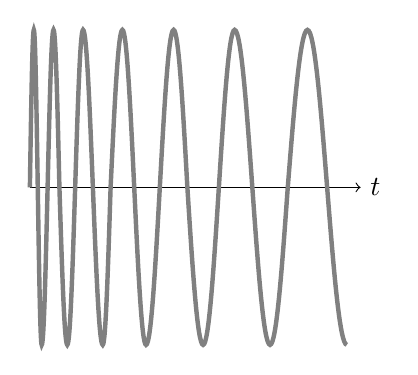
\begin{tikzpicture}
\shorthandoff{<>."}
  \draw[->] (0,0) -- (4.2,0) node[right] {$t$};
  \draw [x=0.5cm,y=2cm, ultra thick, gray] (0,0) 
  sin (0.1,1) cos (0.2,0) sin (0.3,-1) 
  cos (0.45,0) sin (0.6,1) cos (0.75,0) 
  sin (0.95,-1) cos (1.15,0) sin (1.35,1)
  cos (1.6,0) sin (1.85,-1) cos (2.05,0) 
  sin (2.35,1) cos (2.65,0) sin (2.95,-1)
  cos (3.3,0) sin (3.65,1) cos (4,0)
  sin (4.4,-1) cos (4.8,0) sin (5.2,1)
  cos (5.65,0) sin (6.1,-1) cos (6.55,0)
  sin (7.05,1) cos (7.55,0) sin (8.05,-1);
  \shorthandon{<>."}
\end{tikzpicture}
\end{center}
\caption[Frecuencia mayor a menor]{La onda disminuye su frecuencia con la progresi\'on de tiempo $t$.}
\label{fig:freq}
\end{figure}